\documentclass[peerreview,11pt,draftcls,onecolumn]{IEEEtran}

%% Packages
\usepackage{cite}
\usepackage[pdftex]{graphicx} \graphicspath{{images/}}
\usepackage[cmex10]{amsmath}
%\usepackage{algorithm}
\usepackage{algorithmic}
\usepackage{array}
\usepackage{mdwmath}
\usepackage{mdwtab}
\usepackage{eqparbox}
\usepackage[caption=false,font=footnotesize]{subfig}
\usepackage{fixltx2e}
%\usepackage{stfloats}
\usepackage{url}
\usepackage{color}

\newenvironment{meta}[0]{\color{red} \em}{}

% correct bad hyphenation here
\hyphenation{}


\begin{document}

\title{Improved Particle Approximations \\ to the Joint Smoothing Distribution \\ Using Markov Chain Monte Carlo}

\author{Pete~Bunch*,~\IEEEmembership{Member,~IEEE,} and
        Simon~Godsill,~\IEEEmembership{Member,~IEEE}% <-this % stops a space
\thanks{P. Bunch and S. Godsill are with the Department
of Engineering, Cambridge University, UK. email: \{pb404,sjg30\}@cam.ac.uk}% <-this % stops a space
\thanks{Manuscript received April 03, 2012.}}

%% The paper headers
%\markboth{IEEE Transactions on Signal Processing,~Vol.~AA, No.~BB, January~YYYY}%
%{MCMC Particle Smoothing Approximations}

% make the title area
\maketitle


\begin{abstract}
Particle filtering and smoothing algorithms approximate posterior state distributions with a set of samples drawn from those distributions. Conventionally, samples from the joint smoothing distribution are generated by sequentially resampling from the particle filter results. If the number of filtering particles is high, this process is limited by computational complexity. In addition, the support of the smoothing distribution is restricted to the values which appear in the filtering approximation. In this paper, a Metropolis-Hastings sampling procedure is used to improve the efficiency of the particle smoother, achieving comparable error performance but with a lower execution time. In addition, an algorithm for approximating the joint smoothing distribution without limited support is presented, which achieves simultaneous improvements in both execution time and error. These algorithms also provide a greater degree of flexibility over existing methods, allowing a trade-off between execution time and error, controlled by the length of the Markov chains.
\end{abstract}



%\begin{IEEEkeywords}
%state space model, particle filter, smoothing, MCMC, Bayesian inference
%\end{IEEEkeywords}

\ifCLASSOPTIONpeerreview
\begin{center} \bfseries EDICS Categories: MLR-BAYL, SSP-NGAU, SSP-TRAC, SSP-FILT \end{center}
\fi

\newpage
% For peerreview papers, this IEEEtran command inserts a page break and
% creates the second title. It will be ignored for other modes.
%\IEEEpeerreviewmaketitle



\section{Introduction} \label{sec:intro}

\IEEEPARstart{T}{he} objective of sequential Bayesian inference is the estimation of an unknown, time-varying quantity from incomplete or inaccurate observations. This is commonly achieved through the use of discrete-time probabilistic models for the evolution of the latent state and the measurement process, defined by transition and observation densities,
%
\begin{IEEEeqnarray}{rCl}
x_{k} & \sim & p(x_{k}|x_{k-1}) \label{eq:state_proc}\\
y_{k} & \sim & p(y_{k}|x_{k})   \label{eq:observ_proc}   .
\end{IEEEeqnarray}

Here, the random variable $x_k$ denotes the value of the latent state at the $k$th instant, and $y_k$ the value of the observation. A set of random variables will be written as $x_{1:k} = \{x_1, x_2, \dots, x_k \}$. The state evolution is assumed to be Markovian, i.e. $x_k$ depends only on the previous value, $x_{k-1}$.

Commonly of interest are the problems of filtering and smoothing. Filtering is the inference of $p(x_k|y_{1:k})$, the distribution of the current state given all previous observations. Smoothing comprises two related tasks, the inference of $p(x_{1:K}|y_{1:K})$ (where $K$ is the number of time steps), the joint distribution of the entire state sequence given all the observations, and that of $p(x_{k}|y_{1:K})$, the marginal distribution of each state given all the observations. In this paper, we are concerned with the estimation of the joint smoothing distribution.

In the case where the state and observation processes of (\ref{eq:state_proc}) and~(\ref{eq:observ_proc}) are linear and Gaussian, the filtering problem may be solved analytically using the Kalman filter \cite{Kalman1960}. For nonlinear or non-Gaussian models, tractable closed-form solutions are rare. Instead, numerical approximations are often employed, including the particle filter algorithm, first introduced by \cite{Gordon1993}. (See \cite{Cappe2007,Doucet2009} for a thorough introduction.)

In a particle filter, the filtering distribution is approximated by a set of weighted samples (or ``particles'') drawn from that distribution,
%
\begin{IEEEeqnarray}{rCl}
\hat{p}(x_{k}|y_{1:k}) & = & \sum_i w_k^{(i)} \delta_{x_k^{(i)}}(x_k)     .
\end{IEEEeqnarray}

Here, $\delta_{a}(x)$ indicates a discrete probability mass at the point $x = a$, and $w_k^{(i)}$ is the weight of the $i$th particle. Weights are non-negative and sum to 1.% $\hat{p}$ means an approximation to $p$.

Similar ideas apply to the problem of smoothing. In the linear Gaussian case, the entire state sequence, $x_{1:K}$, may be estimated in closed-form using the Rauch-Tung-Striebel (RTS) smoother \cite{Rauch1965}. This works by modifying the ordinary Kalman filter results in a backward processing pass through the state sequence. For nonlinear or non-Gaussian models, it is possible again to resort to numerical methods. Now, particles are used to approximate the joint smoothing distribution,
%
\begin{IEEEeqnarray}{rCl}
\hat{p}(x_{1:K}|y_{1:K}) & = & \sum_i w_K^{(i)} \delta_{x_{1:K}^{(i)}}(x_{1:K})     .
\end{IEEEeqnarray}

Each particle is an entire realisation of the state process, with $K$ values corresponding to the state at each time step. Methods for generating these samples have been described in \cite{Kitagawa1996,Godsill2004,Briers2010}. In this paper new algorithms are presented for drawing samples from the joint smoothing distribution, using Metropolis-Hastings (MH). These novel procedures have computational advantages and greater flexibility over previous methods.

In section~\ref{sec:basics}, we briefly review the basic particle filter and existing joint smoother algorithms. The new MH-based smoothing methods are presented in sections~\ref{sec:mcmc_smoother} and~\ref{sec:new_state_smoother} with supporting simulations in section~\ref{sec:simulations}.



\section{Particle Filtering and Smoothing} \label{sec:basics}

\subsection{The Particle Filter}

The particle filter is a recursive numerical algorithm for estimation of the filtering distribution. At the $k$th processing step, a particle estimate of the joint density over $x_{k-1}$ and $x_k$ is made using importance sampling (IS). A particle is first sampled from the factorised proposal density,
%
\begin{IEEEeqnarray}{rCl}
\{ x_{k-1}^{(i)}, x_k^{(i)} \} & \sim & q(x_{x}|x_{k-1}) q(x_{k-1}).
\end{IEEEeqnarray}

The proposal for $x_k$, $q(x_{x}|x_{k-1})$, is often called the ``importance density''. Common choices for this include the model transition density (\ref{eq:state_proc}), and the ``optimal importance density'' \cite{Doucet2000a}. The proposal density for $x_{k-1}$, $q(x_{k-1})$, is constructed from the particles of the filtering approximation from the previous time step. The choice of weights and sampling procedure for $x_{k-1}$ determine what form of ``resampling'' is to be used. Here we use arbitrary weights for generality,
%
\begin{IEEEeqnarray}{rCl}
q(x_{k-1}) & = & \sum_i v_{k-1}^{(i)} \delta_{x_{k-1}^{(i)}}(x_{k-1})     .
\end{IEEEeqnarray}

The choice $v_{k-1}^{(i)} = w_{k-1}^{(i)}$ corresponds to ordinary resampling, and other choices of $v_{k-1}^{(i)}$ represent auxiliary sampling schemes \cite{Pitt1999,Cappe2007}. For the least computational expense, the proposal density with weights $v_{k-1}^{(i)} = 1/N_F$ (where $N_F$ is the number of filter particles) can be ``sampled'' by simply keeping the set of particles generated in the last step, with no resampling. This, however, leads to degeneracy of the particle weights over time. (See \cite{Cappe2007,Doucet2009} for further discussion of resampling.)

Next, the particles are assigned an importance weight according to the ratio of the target and the proposal densities,
%
\begin{IEEEeqnarray}{rCl}
w_{k}^{(i)} & =       & \frac{ p(x_{k-1}^{(i)}, x_k^{(i)}|y_{1:k}) }{ q(x_{x}^{(i)}|x_{k-1}^{(i)}) q(x_{k-1}^{(i)}) } \nonumber \\
            & \propto & \frac{ p(y_k|x_k^{(i)}) p(x_k^{(i)}|x_{k-1}^{(i)}) p(x_{k-1}^{(i)}|y_{1:k-1}) }{ q(x_{x}^{(i)}|x_{k-1}^{(i)}) q(x_{k-1}^{(i)}) } \nonumber \\
            & =       & \frac{ p(y_k|x_k^{(i)}) p(x_k^{(i)}|x_{k-1}^{(i)}) }{ q(x_{x}^{(i)}|x_{k-1}^{(i)}) } \times \frac{w_{k-1}^{(i)}}{v_{k-1}^{(i)} }     .
\end{IEEEeqnarray}

Normalisation is enforced by scaling the weights so that they sum to 1. Finally, $x_{k-1}$ is marginalised from the distribution by simply discarding the $x_{k-1}^{(i)}$ values from each particle. The particle filter is summarised in Fig.~\ref{alg:PF}.

\begin{figure}
\fbox{\parbox{\columnwidth}{
\begin{algorithmic}[1]
\linespread{1.7} \selectfont
	\STATE Initialise particles from prior, $x_{0}^{(i)} \sim p(x_{0})$.
	\FOR{$k = 1$ \TO $K$}
 		\FOR{$i = 1$ \TO $N_F$}
 		  \STATE Resample last state $x_{k-1}^{(i)} \sim \sum_j v_{k-1}^{(j)} \delta_{x_{k-1}^{(j)}}(x_{k-1})$.
 			\STATE Sample new state $x_k^{(i)} \sim q(x_k|x_{k-1}^{(i)})$.
 			\STATE Weight $w_{k}^{(i)} \propto \frac{ p(y_k|x_k^{(i)}) p(x_k^{(i)}|x_{k-1}^{(i)}) }{ q(x_{x}^{(i)}|x_{k-1}^{(i)}) } \times \frac{w_{k-1}^{(i)}}{v_{k-1}^{(i)} }$.
 			\STATE Discard $x_{k-1}^{(i)}$.
 		\ENDFOR
 	  \STATE Scale weights so that $\sum_i w_{k}^{(i)} = 1$.
 	\ENDFOR
\end{algorithmic}
}}
\caption{Particle filter algorithm}
\label{alg:PF}
\end{figure}

\subsection{Existing Algorithms for Particle Smoothing } \label{sec:existing_smoothers}

The particle filter generates a numerical approximation to each filtering distribution, $p(x_k|y_{1:k})$ by simulating a set of samples from each. A similar sampling-based method may be used to estimate the smoothing distribution.

The most basic particle smoother was presented in \cite{Kitagawa1996}, and is a straightforward extension of the particle filter. Rather than marginalising the previous states from each particle, these past values are stored as well. Thus, at each step the algorithm generates an approximation to $p(x_{1:k}|y_{1:k})$. The output from the final processing step is an approximation to the desired smoothing distribution. This simple filter-smoother is summarised in Fig.~\ref{alg:FS}.

The weakness of the filter-smoother is degeneracy of the particles in the path-space. Every time the particles are resampled, those with low weights do not appear in the approximation at the next step, whereas those with high weights appear multiple times. The result is that many, or even all, particles will share a common ancestor, before which they all have the same set of state values. If the objective is only to produce a single point estimate then this might be sufficient, but to characterise the complete smoothing distribution, the path-space diversity of the approximation must be increased.

\begin{figure}
\fbox{\parbox{\columnwidth}{
\begin{algorithmic}[1]
\linespread{1.7} \selectfont
 	\STATE Initialise particles from prior, $x_{0}^{(i)} \sim p(x_{0})$.
 	\FOR{$k = 1$ \TO $K$}
 		\FOR{$i = 1$ \TO $N_F$}
 			\STATE Resample history $x_{1:k-1}^{(i)} \sim \sum_j v_{k-1}^{(j)} \delta_{x_{1:k-1}^{(j)}}(x_{1:k-1})$.
 			\STATE Sample new state $x_k^{(i)} \sim q(x_k|x_{k-1}^{(i)})$.
 			\STATE Weight $w_{k}^{(i)} \propto \frac{ p(y_k|x_k^{(i)}) p(x_k^{(i)}|x_{k-1}^{(i)}) }{ q(x_{x}^{(i)}|x_{k-1}^{(i)}) } \times \frac{w_{k-1}^{(i)}}{v_{k-1}^{(i)} }$.
 		\ENDFOR
 	  \STATE Scale weights so that $\sum_i w_{k}^{(i)} = 1$.
 	\ENDFOR
\end{algorithmic}
}}
\caption{Filter-smoother algorithm}
\label{alg:FS}
\end{figure}

An improved particle smoother was presented in \cite{Godsill2004}, the forward-filtering-backward-sampling (FFBS) algorithm. This works by constructing new particles from the smoothing distribution by sampling from the filtering approximations. The sampling procedure exploits the following factorisation of the joint distribution,
%
\begin{IEEEeqnarray}{rCl}
p(x_{1:K}|y_{1:K}) & = & p(x_K|y_{1:K}) \prod_{k=1}^{K-1} p(x_k|x_{k+1}, y_{1:K}) \label{eq:smoothing_factorisation}     .
\end{IEEEeqnarray}

Particles are generated by sampling backwards in time from the factors of this expansion. At the $k$th step, a sample $\tilde{x}_{k+1:K} \sim p(x_{k+1:K}|y_{1:K})$ will already have been drawn. By sampling $x_k \sim p(x_k|\tilde{x}_{k+1}, y_{1:K})$ and appending $x_k$ to $\tilde{x}_{k+1:K}$, the state sequence is sequentially extended back in time. The recursion is initialised with $x_K \sim p(x_K|y_{1:K})$, i.e. a sample from the final filtering approximation.

The backwards conditional density may be expanded with Bayes' rule,
%
\begin{IEEEeqnarray}{rCl}
p(x_k|\tilde{x}_{k+1}, y_{1:K}) & =       & p(x_k|\tilde{x}_{k+1}, y_{1:k}) \nonumber \\
                                & \propto & p(\tilde{x}_{k+1}|x_k) p(x_k|y_{1:k})   .
\end{IEEEeqnarray}

Substituting the filtering approximation into this expression yields a particle distribution which may be sampled easily,
%
\begin{IEEEeqnarray}{rCl}
\hat{p}(x_k|\tilde{x}_{k+1}, y_{1:K}) = \sum_i  \tilde{w}_k^{(i)} \delta_{x_{k}^{(i)}}(x_{k}) \label{eq:backward_conditional_filter} \\
\tilde{w}_k^{(i)} \propto w_k^{(i)} p(\tilde{x}_{k+1}|x_k^{(i)}) \label{eq:DBRS_weights}     .
\end{IEEEeqnarray}

The procedure may be repeated to produce as many samples from the joint smoothing distribution as required. In this paper, we refer to this algorithm as the direct FFBS (D-FFBS) algorithm, in order to distinguish it from the MH variant developed in the next section. The D-FFBS algorithm is summarised in Fig.~\ref{alg:DBRS}.

\begin{figure}
\fbox{\parbox{\columnwidth}{
\begin{algorithmic}[1]
\linespread{1.7} \selectfont
 	\STATE Run a particle filter to approximate $p(x_k|y_{1:k})$ for each $k$ and store the resulting particles $\{x_k^{(i)}, w_k^{(i)}\}$.
	\FOR{$i = 1$ \TO $N_S$}
		\STATE Sample $\tilde{x}_{K}^{(i)} \sim \sum_j w_K^{(j)} \delta_{x_{K}^{(j)}}(x_{K})$.
		\FOR{$k = K-1$ \TO $1$}
			\FOR{$j = 1$ \TO $N_F$}
				\STATE Calculate weight $\tilde{w}_k^{(j)} = w_k^{(j)} p(\tilde{x}_{k+1}|x_k^{(j)})$.
			\ENDFOR
			\STATE Sample $\tilde{x}_{k}^{(i)} \sim \sum_j \tilde{w}_k^{(j)} \delta_{x_{k}^{(j)}}(x_{k})$.
		\ENDFOR
	\ENDFOR
\end{algorithmic}
}}
\caption{Direct forward-filtering-backward-sampling algorithm}
\label{alg:DBRS}
\end{figure}

A method for drawing samples from the joint smoothing distribution, $p(x_{1:K}|y_{1:K})$, is included in \cite{Briers2010}. The principal topic of this paper is a two-filter smoother for estimation of the marginal smoothing distributions, $p(x_{k}|y_{1:K})$, by combination of the results from one forward and one backward particle filter. Particles from the joint distribution may then be generated by resampling from either the forward or backward filters (or some combination) in the manner of the D-FFBS algorithm outlined above.

The complexity of both the D-FFBS smoother of \cite{Godsill2004} and the two-filter variant of \cite{Briers2010} is $\mathcal{O}(N_F \times N_S \times K)$, where $N_F$ is the number of filter particles, $N_S$ the number of smoother particles, and $K$ the number of time steps. In \cite{Douc2009}, a theoretically linear-cost scheme using rejection sampling is outlined. In practice this often appears to be slower than the standard algorithms when there are more than a few state dimensions, due to high rejection rates. Methods for reducing the computational complexity of smoothing algorithms are also discussed in \cite{Klaas2006}. However, these focus on approximating a sum of kernel values over a set of particles, such as those which arise in forward-backward-smoothing \cite{Doucet2000a} and two-filter smoothing \cite{Briers2010} for estimation of the marginal smoothing distributions. They are not applicable for the joint smoothing procedures.

In the algorithms described so far, no new states are sampled during the backwards smoothing pass; state values are only ``recycled'' from the particle filtering approximations. This limits the support of the smoother to the states that appear in these filtering particles. In \cite{Fearnhead2010}, an IS-based algorithm for estimation of the marginal smoothing distributions is described in which new states are sampled from a proposal density, thus recovering the full support. In addition, this algorithm achieves $\mathcal{O}( N_S \times K)$ complexity, i.e. linear in the number of particles.



\section{An MCMC Particle Smoother} \label{sec:mcmc_smoother}

The bottleneck of the D-FFBS algorithm is the calculation of the sampling weights, specified by (\ref{eq:DBRS_weights}). For each smoother particle and for each time step, a weight must be calculated for each of the $N_F$ filter particles, in order to draw a sample from the conditional distribution $\hat{p}(x_k|\tilde{x}_{k+1}, y_{1:K})$. The innovation here is to use a Markov chain Monte Carlo (MCMC) procedure to produce these particles instead of sampling directly.

MCMC algorithms are a class of numerical procedures which use a Markov chain to draw dependent samples from a target probability distribution. A thorough introduction can be found in \cite{Gilks1996}. The basic Metropolis-Hastings (MH) \cite{Hastings1970} sampler uses a series of steps in which a new state is drawn from a proposal distribution and accepted with a probability determined by the ratios of the target and proposal densities.

For the D-FFBS, the objective at each time step was to draw a sample from $p(x_{k}|\tilde{x}_{k+1}, y_{1:K})$. To simplify the notation and initialisation of chains, the MH version will target $p(x_{1:k}|\tilde{x}_{k+1}, y_{1:K})$. Theoretically this means using the particles of the filter-smoother, $\{x_{1:k}^{(i)}\}$, rather than just the filter, $\{x_k^{(j)}\}$, which would require $\mathcal{O}(K^2)$ memory. However, as discussed later, this is not required in practice.

As before, the algorithm begins by first running a particle filter-smoother and then resampling states backwards through time to produce particles from the joint smoothing distribution, using the factorisation of (\ref{eq:smoothing_factorisation}). At the $k$th time step, a Markov chain is used to sample from $p(x_{1:k}|\tilde{x}_{k+1}, y_{1:K})$. The chain is initialised with the output from the previous processing step. As this is itself a sample from the target distribution, no burn-in period is required.

Following an equivalent derivation to that for (\ref{eq:backward_conditional_filter}), the target distribution may be approximated by a set of particles,
%
\begin{IEEEeqnarray}{rCl}
\hat{p}(x_{1:k}|\tilde{x}_{k+1}, y_{1:K}) = \sum_i  \tilde{w}_k^{(i)} \delta_{x_{1:k}^{(i)}}(x_{1:k}) \\
\tilde{w}_k^{(i)} \propto w_k^{(i)} p(\tilde{x}_{k+1}|x_k^{(i)}) \label{eq:MCMC-BRS_weights}   .
\end{IEEEeqnarray}

A valid proposal may be constructed using the particles of the filter-smoother approximation with any arbitrary weights,
%
\begin{IEEEeqnarray}{rCl}
q(x_{1:k}|\tilde{x}_{k+1}, y_{1:K}) & = & \sum_j \tilde{v}_k^{(j)} \delta_{x_{1:k}^{(j)}}(x_{1:k})     .
\end{IEEEeqnarray}

If the current state of the chain is $x_{1:k}^{(m)}$, and a new sample is drawn from the proposal $x_{1:k}^{*} \sim q(x_{1:k}|\tilde{x}_{k+1}, y_{1:K})$, then it should be accepted with the following probability,
%
\begin{IEEEeqnarray}{rCl}
\alpha &=& \min \Bigg[ 1, \frac{ \hat{p}(x_{1:k}^{*}|\tilde{x}_{k+1}, y_{1:K}) q(x_{1:k}^{(m)}|\tilde{x}_{k+1}, y_{1:K}) }{ \hat{p}(x_{1:k}^{(m)}|\tilde{x}_{k+1}, y_{1:K}) q(x_{1:k}^{*}|\tilde{x}_{k+1}, y_{1:K}) } \Bigg] \nonumber \\
       &=& \min \Bigg[1, \frac{ w_k^{*} \tilde{v}_k^{(m)} }{  w_k^{(m)} \tilde{v}_k^{*} } \times \frac{ p(\tilde{x}_{k+1}|x_k^{*}) }{ p(\tilde{x}_{k+1}|x_k^{(m)}) }  \Bigg]  . \label{eq:MCMC-BRS_ap}
\end{IEEEeqnarray}

Note that $w_k^{*}$ indicates the filtering particle weight of the proposed new state, $x_{1:k}^{*}$. The final state of each chain is used as a sample from the required conditional distribution. The resulting MH-FFBS algorithm is summarised in Fig.~\ref{alg:MCMC-BRS}.

\begin{figure}
\fbox{\parbox{\columnwidth}{
\begin{algorithmic}[1]
\linespread{1.7} \selectfont
 	\STATE Run a particle filter to approximate $p(x_{1:k}|y_{1:k})$ for each $k$ and store the resulting particles $\{x_{1:k}^{(i)}, w_k^{(i)}\}$.
	\FOR{$i = 1$ \TO $N_S$}
		\STATE Sample $\tilde{x}_{1:K}^{(i)} \sim \sum_j w_K^{(j)} \delta_{x_{1:K}^{(j)}}(x_{1:K})$.
		\FOR{$k = K-1$ \TO $1$}
			\STATE $x_{1:k}^{(i)(0)} \gets \tilde{x}_{1:k}^{(i)}$.
			\FOR{$m = 1$ \TO $M$}
				\STATE Propose a new state, $x_{1:k}^{(i)*} \sim \sum_j \tilde{v}_k^{(j)} \delta_{x_{1:k}^{(j)}}(x_{1:k})$.
				\STATE With probability $\alpha$ specified by (\ref{eq:MCMC-BRS_ap}),\\ $x_{1:k}^{(i)(m)} \gets x_{1:k}^{(i)*}$. Otherwise, $x_{1:k}^{(i)(m)} \gets x_{1:k}^{(i)(m-1)}$.
			\ENDFOR
			\STATE $\tilde{x}_{1:k}^{(i)} \gets x_{1:k}^{(i)(M)}$
		\ENDFOR
	\ENDFOR
\end{algorithmic}
}}
\caption{Metropolis-Hastings forward-filtering-backward-sampling algorithm}
\label{alg:MCMC-BRS}
\end{figure}

For a practical implementation, it is not necessary to store the complete particles of the filter-smoother approximations, $\hat{p}(x_{1:k}|y_{1:k})$, which would require memory space which scaled quadratically with $K$. As the smoother progresses backwards in time, the earlier states in the sequence are repeatedly overwritten, and so it is not necessary ever to have known them. Thus, it is only necessary to store the last two states in each filter-smoother particle (i.e. $\{x_{k-1}^{(j)}\}$ and $\{x_{k}^{(j)}\}$).

The computational complexity of the MH-based algorithm is $\mathcal{O}(M \times N_S \times K)$, where $M$ is the (mean) number of MH steps used for each time step and smoothing particle. The advantage of the new procedure is that $M$ can often be much smaller than $N_F$ and yet achieve almost equal error performance.

With the D-FFBS, the only parameter to be chosen is $N_S$, the number of smoother particles. With the MH variant, we also have the freedom to set $M$, the number of MH steps in each Markov chain. This controls a trade-off between speed and accuracy/particle diversity. If the chains are short, and the acceptance probabilities low, then this scheme will simply reproduce particles from the filter-smoother. However, when the weights of the conditional distribution approximation (\ref{eq:MCMC-BRS_weights}) are similar, then an independent sample may be produced with only a very short chain.

The new scheme targets the same empirical approximation to the smoothing distribution as used in the D-FFBS method. However, rather than drawing independent samples from this approximation, MH is used, resulting in dependent samples.  In the limit as the number of MH steps, $M$, tends to infinity, the Markov chain will produce an independent sample from the target distribution, as the initial state of the chain will have been forgotten. At this point, the performance of the MH method is expected to match that of the direct method in terms of error and particle diversity. At the other extreme, with $M=0$, the algorithm simply outputs particles from the filter-smoother approximation, which is expected to give worse performance. With intermediate values of $M$, the quality of the approximation is expected to fall between those of the filter-smoother and direct backward-resampling smoother.

This new scheme bears a resemblance to the ``linear cost'' simulation scheme of \cite{Douc2009} which uses rejection sampling instead of MH. Although theoretically elegant, the latter algorithm has been found to suffer from such high rejection rates as to render it consistently slower than the direct sampling implementation on problems with more than one state dimension (see section~\ref{sec:simulations}).



\section{An MCMC particle smoother with improved support} \label{sec:new_state_smoother}

The FFBS smoothers, both the direct sampling version of \cite{Godsill2004} and the MH version outlined in the previous section, are limited by the fact that states are only selected from those which appear in the filtering approximation. If there is a significant difference between the filtering and smoothing densities, then the particles are unlikely to be in the right locations to represent the smoothing distribution well, and the resulting approximation will be poor.

In \cite{Fearnhead2010}, the authors described an algorithm for estimating the marginal smoothing distributions. For this method, states were proposed afresh rather than simply resampling from the filtering approximations. This yielded improvements in accuracy and particle diversity over other marginal smoothing techniques, and also the advantage of $\mathcal{O}(N_S \times K)$ complexity. Here we adapt this method for generating particles from the joint smoothing distribution. Again, an MCMC procedure is employed.

The smoother described in \cite{Fearnhead2010} uses importance sampling to approximate the marginal smoothing distributions. This method could be extended to estimation of the joint smoothing distribution by applying it sequentially. However, the resampling required to limit weight degeneracy would lead to a loss of path-space diversity similar to that suffered by the filter-smoother.

The proposed new method proceeds in a similar manner to the MH-FFBS algorithm. However, this time only $x_{1:k-1}$ is resampled from the particle filter-smoother approximation from time step $k-1$. The current state, $x_k$, is then sampled afresh from a new proposal distribution. Thus the factorised proposal may be written as follows,
%
\begin{IEEEeqnarray}{rCl}
\IEEEeqnarraymulticol{3}{l}{ q(x_{1:k}|\tilde{x}_{k+1}, y_{1:K}) = q(x_{1:k-1}|y_{1:k-1}) q(x_{k}|x_{k-1}, \tilde{x}_{k+1}, y_{k}) } \nonumber \\
                                    & = & \sum_j \tilde{v}_{k-1}^{(j)} \delta_{x_{1:k-1}^{(j)}}(x_{1:k-1}) q(x_{k}|x_{k-1}^{(j)}, \tilde{x}_{k+1}, y_{k})  .
\end{IEEEeqnarray}

The target distribution is also factorised,
%
\begin{IEEEeqnarray}{rCl}
\IEEEeqnarraymulticol{3}{l}{p(x_{1:k}|\tilde{x}_{k+1}, y_{1:K}) = p(x_{1:k}|\tilde{x}_{k+1}, y_{1:k}) } \nonumber \\
                                    & \propto & p(\tilde{x}_{k+1}|x_k) p(x_k|x_{k-1}) p(y_k|x_x) p(x_{1:k-1}|y_{1:k-1})     .
\end{IEEEeqnarray}

Using the filter-smoother approximation for $p(x_{1:k-1}|y_{1:k-1})$, the MH acceptance probabilities may then be calculated,
%
\begin{IEEEeqnarray}{rCl}
\alpha &=& \min \Bigg[ 1, \frac{ \hat{p}(x_{1:k}^{*}|\tilde{x}_{k+1}, y_{1:K}) q(x_{1:k}^{(m)}|\tilde{x}_{k+1}, y_{1:K}) }{ \hat{p}(x_{1:k}^{(m)}|\tilde{x}_{k+1}, y_{1:K}) q(x_{1:k}^{*}|\tilde{x}_{k+1}, y_{1:K}) } \Bigg] \nonumber \\
 &=& \min \Bigg[ 1, \frac{ w_{k-1}^{*} p(\tilde{x}_{k+1}|x_k^{*}) p(x_k^{*}|x_{k-1}^{*}) p(y_k|x_k^{*}) }{ w_{k-1}^{(m)} p(\tilde{x}_{k+1}|x_k^{(m)}) p(x_k^{(m)}|x_{k-1}^{(m)}) p(y_k|x_k^{(m)}) } \nonumber \\
 & & \times \frac{ \tilde{v}_{k-1}^{(m)} q(x_k^{(m)}|x_{k-1}^{(m)},\tilde{x}_{k+1},y_k) }{ \tilde{v}_{k-1}^{*} q(x_k^{*}|x_{k-1}^{*},\tilde{x}_{k+1},y_k) } \Bigg] \label{eq:MCMC-BSS_ap}     .
\end{IEEEeqnarray}

We refer to this algorithm as the Metropolis-Hastings forward-filtering-backward-proposing (MH-FFBP) smoother, emphasising the fact that samples are proposed afresh rather than recycling those from the filtering approximations. The complete algorithm is summarised in Fig.~\ref{alg:MCMC-BSS}. The computational complexity of this algorithm is $\mathcal{O}(M \times N_S \times K)$, the same as the MH-FFBS smoother, although it is likely take more time to run because of the additional sampling operation and probability calculations. In contrast with the MH-FFBS algorithm, this smoother targets the exact posterior distribution for the current state at time $t_n$, rather than a particle approximation. Consequently, the performance is expected to be improved relative to the FFBS methods in terms of both error and particle diversity.

We note that the MH-FFBP algorithm shares similar features with the procedure published recently in \cite{Dubarry2011}. The latter iteratively applies MH steps to a particle approximation of the joint smoothing algorithm in order to improve particle diversity. In this sense, it is akin to a resample-move \cite{Gilks2001} scheme for the entire smoothing distribution. In contrast, the MH-FFBP algorithm integrates MH steps into a single backward smoothing pass. It allows changes to the entire state history of a particle by proposing $x_{1:k-1}$ from the filtering approximation.

\begin{figure}
\fbox{\parbox{\columnwidth}{
\begin{algorithmic}[1]
\linespread{1.7} \selectfont
 	\STATE Run a particle filter to approximate $p(x_{1:k}|y_{1:k})$ for each $k$.
	\FOR{$i = 1$ \TO $N_S$}
		\STATE Sample $\tilde{x}_{1:K}^{(i)} \sim \sum_j w_K^{(j)} \delta_{x_{1:K}^{(j)}}(x_{1:K})$.
		\FOR{$k = K-1$ \TO $1$}
			\STATE $x_{1:k}^{(i)(0)} \gets \tilde{x}_{1:k}^{(i)}$.
			\FOR{$m = 1$ \TO $M$}
				\STATE Propose a new state history,\\ $x_{1:k-1}^{(i)*} \sim \sum_j \tilde{v}_{k-1}^{(j)} \delta_{x_{1:k-1}^{(j)}}(x_{1:k-1})$.
				\STATE Propose a new state, $x_{k}^{(i)*} \sim q(x_k|x_{k-1}^{*},\tilde{x}_{k+1},y_k)$.
				\STATE With probability $\alpha$ specified by (\ref{eq:MCMC-BSS_ap}),\\ $x_{1:k}^{(i)(m)} \gets x_{1:k}^{(i)*}$. Otherwise, $x_{1:k}^{(i)(m)} \gets x_{1:k}^{(i)(m-1)}$.
			\ENDFOR
			\STATE $\tilde{x}_{1:k}^{(i)} \gets x_{1:k}^{(i)(M)}$
		\ENDFOR
	\ENDFOR
\end{algorithmic}
}}
\caption{Metropolis-Hastings forward-filtering-backward-proposing algorithm}
\label{alg:MCMC-BSS}
\end{figure}



\subsection{Proposal Densities}

When using MH, if samples can be proposed directly from the target distribution then the acceptance probability is always 1 (In combination with a block-sampling scheme, this becomes the Gibbs sampler of \cite{geman1984}). This is desirable as it maximises the acceptance rate. Clearly, for the basic MH-FFBS smoother of section~\ref{sec:mcmc_smoother}, such a ``target density proposal'' simply yields the D-FFBS smoother of \cite{Godsill2004}, as described in section~\ref{sec:existing_smoothers}. For the MH-FFBP smoother, a target density proposal can be made by sequentially sampling $x_{1:k-1}$ followed by $x_k$ using the following factorisation,
%
\begin{IEEEeqnarray}{rCl}
\IEEEeqnarraymulticol{3}{l}{p(x_{1:k}|\tilde{x}_{k+1}, y_{1:K}) = p(x_{1:k}|\tilde{x}_{k+1}, y_{1:k}) } \nonumber \\
                                    & \propto & p(x_k|x_{k-1}, \tilde{x}_{k+1}, y_k) p(x_{1:k-1}|y_{1:k}, \tilde{x}_{k+1})   .
\end{IEEEeqnarray}

A good choice for the $x_k$ proposal is thus given by,
%
\begin{IEEEeqnarray}{rCl}
q(x_k|x_{k-1}, \tilde{x}_{k+1}, y_k) & = & p(x_k|x_{k-1}, \tilde{x}_{k+1}, y_k)   .
\end{IEEEeqnarray}

The matching $x_{1:k-1}$ proposal can be approximated using the filter-smoother particles,
%
\begin{IEEEeqnarray}{rCl}
q(x_{1:k-1}|y_{1:k}, \tilde{x}_{k+1}) & =       & p(x_{1:k-1}|y_{1:k}, \tilde{x}_{k+1}) \nonumber \\
                                      & \propto & p(y_{k}, \tilde{x}_{k+1}| x_{1:k-1}) p(x_{1:k-1}|y_{1:k-1}) \nonumber \\
                                      & \approx & \sum_j \tilde{v}_{k-1}^{(j)} \delta_{x_{1:k-1}^{(j)}}(x_{1:k-1})
\end{IEEEeqnarray}
%
\begin{IEEEeqnarray}{rCl}
\tilde{v}_{k-1}^{(j)} & = & w_{k-1}^{(j)} p(y_{k}, \tilde{x}_{k+1}| x_{1:k-1}^{(j)})      .
\end{IEEEeqnarray}

The $x_k$ proposal density may be approximated with linear-Gaussian dynamics, e.g. using an extended \cite{Grewal2002} or unscented \cite{Julier2004} Kalman filter. The weights for the $x_{1:k-1}$ proposal may be approximated using similar methods, but this will often be undesirable. If it is necessary to calculate proposal weights for all of the filter-smoother particles, then the computational advantages of using MH are lost. With this in mind, an appropriate choice for the proposal weights might be simply $\tilde{v}_{k-1}^{(j)} = w_{k-1}^{(j)}$, which avoids calculation of $p(y_{k}, \tilde{x}_{k+1}| x_{1:k-1}^{(j)})$ for all $j$.


\section{Simulations} \label{sec:simulations}

The performance of the new smoothers was tested on a simple 2D tracking model. The trajectory of a single target was simulated using linear-Gaussian dynamics and observed via a nonlinear radar-type measurement model (see \cite{Bar-Shalom2002} for details),
%
\begin{IEEEeqnarray}{rCl}
\underbrace{\begin{bmatrix}x_k \\ y_k \\ \dot{x}_k \\ \dot{y}_k\end{bmatrix}}_{\mathbf{x}_k} &=& \begin{bmatrix}I_2 & \Delta t I_2 \\ 0_2 & I_2\end{bmatrix} \underbrace{\begin{bmatrix}x_{k-1} \\ y_{k-1} \\ \dot{x}_{k-1} \\ \dot{y}_{k-1}\end{bmatrix}}_{\mathbf{x}_{k-1}} + \underbrace{\begin{bmatrix}w_{1,k} \\ w_{2,k} \\ w_{3,k} \\ w_{4,k}\end{bmatrix}}_{\mathbf{w}_k} \\
\underbrace{\begin{bmatrix}b_k \\ r_x\end{bmatrix}}_{\mathbf{y}_k} &=& \begin{bmatrix}\tan^{-1}(y_k / x_k) \\ \sqrt{x_k^2+y_k^2} \end{bmatrix} + \underbrace{\begin{bmatrix}v_{1,k} \\ v_{2,k}\end{bmatrix}}_{\mathbf{v}_k}     .
\end{IEEEeqnarray}

The time between successive time steps is $\Delta t$. $I_2$ and $0_2$ denote the $2 \times 2$ identity and zero matrices respectively. The random variables $\mathbf{w}_k$ and $\mathbf{v}_k$ are independent and are zero-mean Gaussian distributed with covariance matrices $\mathbf{Q}$ and $\mathbf{R}$ respectively,
%
\begin{IEEEeqnarray}{rCl}
\mathbf{Q} &=& \sigma^2_P \begin{bmatrix}\frac{\Delta t^3}{3} I_2 & \frac{\Delta t^2}{2} I_2 \\ \frac{\Delta t^2}{2} I_2 & \Delta t I_2 \end{bmatrix} \\
\mathbf{R} &=& \begin{bmatrix}\sigma^2_B & 0 \\ 0 & \sigma^2_R\end{bmatrix}     .
\end{IEEEeqnarray}

The following algorithms were all implemented for comparison in MATLAB:

\begin{itemize}
	\item The simple filter-smoother (FS) of \cite{Kitagawa1996}
	\item The direct forward-filtering-backward-sampling smoother (D-FFBS) of \cite{Godsill2004}
	\item The new Metropolis-Hastings forward-filtering-backward-sampling smoother (MH-FFBS) of section~\ref{sec:mcmc_smoother}, with several values of $M$
	\item The new Metropolis Hastings forward-filtering-backward-proposing smoother (MH-FFBP) of section~\ref{sec:new_state_smoother}, with several values of $M$
\end{itemize}

The rejection-sampling version of the FFBS described by \cite{Douc2009} was also implemented, but high rejection rates meant that it was impractically slow so it was omitted from further testing.

The algorithms were all used to generate 100 particles from the joint smoothing distribution, using particle filters with 100 particles. Where appropriate, proposal weights were chosen to be equal to filtering weights, i.e. $v_k^{(j)} = w_k^{(j)}$. The particle filter uses the ``optimal importance density'' and the MH-FFBP a ``target density proposal'' with linearisations of the observation model where appropriate.

100 realisations of 500 time steps were simulated from the model and the algorithms tested on each one. Results are shown here for three noise parameter sets. For case 1, the observation variances were set to $\sigma_B^2 = (\pi/720)^2$ and $\sigma_R^2 = 0.1$. For case 2, $\sigma_B^2 = (\pi/36)^2$ and $\sigma_R^2 = 0.1$, resulting in a highly skewed likelihood function. For case 3, $\sigma_B = (\pi/36)^2$ and $\sigma_R^2 = 100$. Other model settings are $\Delta t = 1$, $\sigma_P = 1$, and $x_0 = [-100, 50, 10, 0]^T$. Example trajectories and observations from the two cases are shown in Fig.~\ref{fig:example_trajectories}.

\begin{figure}[!t]
\centering
\subfloat[Case 1]{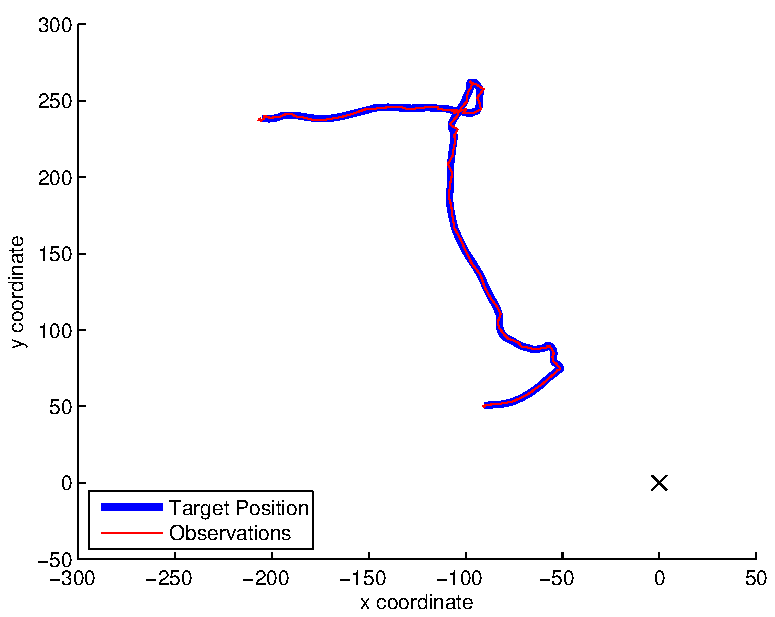
\includegraphics[width=0.45\columnwidth]{case1_trajectory.pdf}}
\\
\subfloat[Case 2]{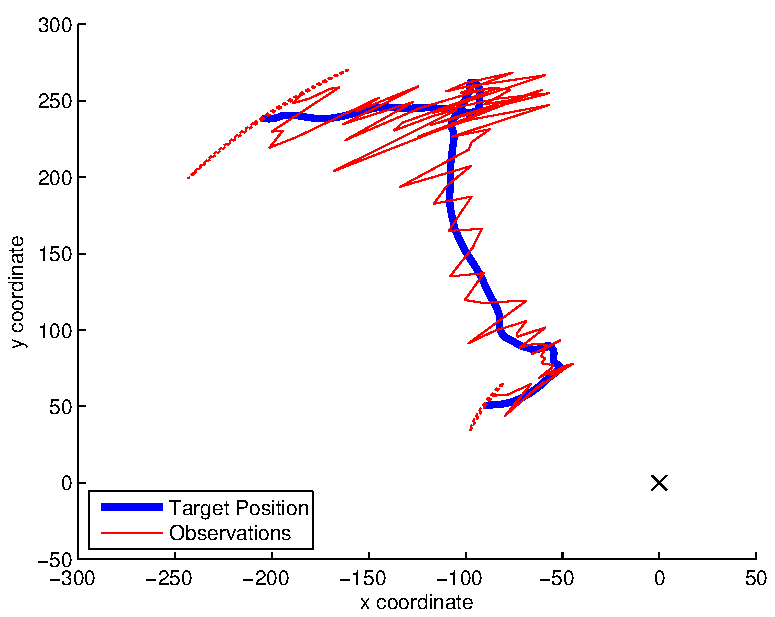
\includegraphics[width=0.45\columnwidth]{case2_trajectory.pdf}}
\\
\subfloat[Case 3]{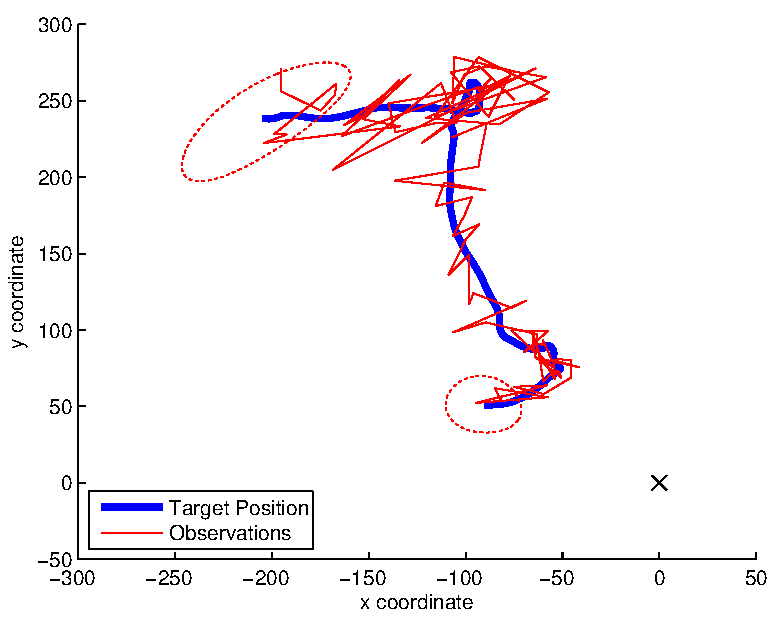
\includegraphics[width=0.45\columnwidth]{case3_trajectory.pdf}}
\caption{Example trajectory with observations from the two noise covariance cases. Constant likelihood contours are shown for the first and last position (dashed)}
\label{fig:example_trajectories}
\end{figure}

The performances of the various smoothing algorithms are compared using a number of measures. At each time point, a single state estimate is calculated by taking the mean of the values from each particle. These point estimates are then used to calculate a root-mean-square error (RMSE). In addition, an empirical normalised estimation error squared (ENEES) is calculated using,
%
\begin{IEEEeqnarray}{rCl}
 \text{ENEES}_k & = & (\hat{\mathbf{x}}_k - \mathbf{x}_k^*)^T \hat{P}_k^{-1} (\hat{\mathbf{x}}_k - \mathbf{x}_k^*) \nonumber \\
 \hat{\mathbf{x}}_k & = & \frac{1}{N_S} \sum_i \mathbf{x}_k^{(i)} \nonumber \\
 \hat{P}_k & = & \frac{1}{N_S} \sum_i (\mathbf{x}^{(i)}_k - \mathbf{x}_k^*) (\mathbf{x}^{(i)}_k - \mathbf{x}_k^*)^T
\end{IEEEeqnarray}

\noindent and where $\mathbf{x}_k^*$ is the true value of the state. This statistic has a value of $1$ when there are fewer linearly independent state values in the particle approximation than state dimensions. It decreases as the number of independent particles increases (improving the covariance estimate) or the estimation error decreases. Thus, it provides a simple relative measure of the quality of different particle approximations, taking into account both estimation error and particle diversity. Finally, the mean number of unique particles at each time instant and the running times (excluding the time for filtering) are also recorded. These performance indicators are all shown in tables~\ref{tab:case1_performance}--\ref{tab:case3_performance} for the two noise scenarios. The trade-off between speed and error is shown in Fig.~\ref{fig:rmse_vs_time}.

\begin{table}[!t]%
\renewcommand{\arraystretch}{1.3}
\caption{Smoother performance measures for noise covariance case 1. All results are averaged over 100 runs, with 500 time steps in each run.}
\label{tab:case1_performance}
{\scriptsize
\begin{center}
\begin{tabular}{|c||c|c|c|c|c|}
\hline
Algorithm & \begin{minipage}[c]{0.9cm} Position RMSE \end{minipage} & \begin{minipage}[c]{0.9cm}  Velocity RMSE \end{minipage} & \begin{minipage}[c]{0.9cm}  ENEES \end{minipage} & \begin{minipage}[c]{0.9cm}  Running Time (s) \end{minipage} & \begin{minipage}[c]{0.9cm}  Unique Particles \end{minipage} \\
\hline
FS             & 0.56 & 0.96 & 0.99 & 0.00 & 2.13 \\
D-FFBS         & 0.45 & 0.76 & 0.84 & 65.88 & 20.54 \\
\hline
MH-FFBS (1)    & 0.48 & 0.81 & 0.90 & 1.80 & 13.95 \\
MH-FFBS (3)    & 0.46 & 0.78 & 0.87 & 3.89 & 17.63 \\
MH-FFBS (10)   & 0.46 & 0.77 & 0.85 & 11.20 & 19.83 \\
MH-FFBS (30)   & 0.45 & 0.76 & 0.84 & 32.05 & 20.40 \\
MH-FFBS (100)  & 0.45 & 0.76 & 0.84 & 105.12 & 20.55 \\
\hline
MH-FFBP (1)    & 0.45 & 0.75 & 0.82 & 9.20 & 44.32 \\
MH-FFBP (3)    & 0.43 & 0.73 & 0.79 & 19.23 & 70.12 \\
MH-FFBP (10)   & 0.43 & 0.72 & 0.78 & 54.33 & 90.10 \\
MH-FFBP (30)   & 0.42 & 0.71 & 0.79 & 154.47 & 96.89 \\
MH-FFBP (100)  & 0.42 & 0.70 & 0.79 & 504.58 & 98.53 \\
\hline
\end{tabular}
\end{center}
}
\end{table}

\begin{table}[!t]%
\renewcommand{\arraystretch}{1.3}
\caption{Smoother performance measures for noise covariance case 2. All results are averaged over 100 runs, with 500 time steps in each run.}
\label{tab:case2_performance}
{\scriptsize
\begin{center}
\begin{tabular}{|c||c|c|c|c|c|}
\hline
Algorithm & \begin{minipage}[c]{0.9cm} Position RMSE \end{minipage} & \begin{minipage}[c]{0.9cm}  Velocity RMSE \end{minipage} & \begin{minipage}[c]{0.9cm}  ENEES \end{minipage} & \begin{minipage}[c]{0.9cm}  Running Time (s) \end{minipage} & \begin{minipage}[c]{0.9cm}  Unique Particles \end{minipage} \\
\hline
FS             & 8.01 & 1.90 & 0.99 & 0.00 & 2.75 \\
D-FFBS         & 7.71 & 1.70 & 0.92 & 66.40 & 14.06 \\
\hline
MH-FFBS (1)    & 7.91 & 1.83 & 0.98 & 1.79 & 6.51 \\
MH-FFBS (3)    & 7.83 & 1.78 & 0.96 & 3.86 & 8.63 \\
MH-FFBS (10)   & 7.77 & 1.73 & 0.93 & 11.09 & 11.39 \\
MH-FFBS (30)   & 7.75 & 1.71 & 0.92 & 31.77 & 13.14 \\
MH-FFBS (100)  & 7.70 & 1.70 & 0.92 & 104.14 & 13.88 \\
\hline
MH-FFBP (1)    & 7.75 & 1.72 & 0.92 & 9.25 & 22.97 \\
MH-FFBP (3)    & 7.67 & 1.67 & 0.88 & 19.34 & 42.22 \\
MH-FFBP (10)   & 7.62 & 1.63 & 0.85 & 54.61 & 70.06 \\
MH-FFBP (30)   & 7.60 & 1.61 & 0.84 & 155.38 & 88.81 \\
MH-FFBP (100)  & 7.59 & 1.60 & 0.84 & 507.58 & 96.82 \\
\hline
\end{tabular}
\end{center}
}
\end{table}

\begin{table}[!t]%
\renewcommand{\arraystretch}{1.3}
\caption{Smoother performance measures for noise covariance case 3. All results are averaged over 100 runs, with 500 time steps in each run.}
\label{tab:case3_performance}
{\scriptsize
\begin{center}
\begin{tabular}{|c||c|c|c|c|c|}
\hline
Algorithm & \begin{minipage}[c]{0.9cm} Position RMSE \end{minipage} & \begin{minipage}[c]{0.9cm}  Velocity RMSE \end{minipage} & \begin{minipage}[c]{0.9cm}  ENEES \end{minipage} & \begin{minipage}[c]{0.9cm}  Running Time (s) \end{minipage} & \begin{minipage}[c]{0.9cm}  Unique Particles \end{minipage} \\
\hline
FS            & 7.41 & 2.15 & 0.98 & 0.00 & 3.97 \\
D-FFBS        & 7.19 & 2.03 & 0.97 & 66.27 & 7.48 \\
\hline
MH-FFBS (1)   & 7.39 & 2.14 & 0.98 & 1.75 & 4.79 \\
MH-FFBS (3)   & 7.36 & 2.12 & 0.98 & 3.75 & 5.33 \\
MH-FFBS (10)  & 7.30 & 2.08 & 0.98 & 10.78 & 6.16 \\
MH-FFBS (30)  & 7.24 & 2.05 & 0.97 & 30.83 & 6.88 \\
MH-FFBS (100) & 7.20 & 2.04 & 0.97 & 101.02 & 7.38 \\
\hline
MH-FFBP (1)   & 7.22 & 2.05 & 0.97 & 9.12 & 12.57 \\
MH-FFBP (3)   & 7.08 & 1.98 & 0.94 & 19.01 & 22.78 \\
MH-FFBP (10)  & 6.95 & 1.92 & 0.92 & 53.64 & 44.15 \\
MH-FFBP (30)  & 6.87 & 1.88 & 0.90 & 152.42 & 70.71 \\
MH-FFBP (100) & 6.84 & 1.86 & 0.88 & 498.38 & 91.35 \\
\hline
\end{tabular}
\end{center}
}
\end{table}


\begin{figure}[!t]
\centering
\subfloat[Case 1]{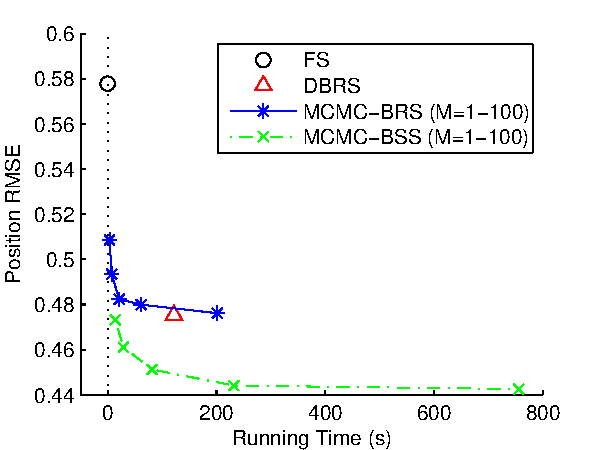
\includegraphics[width=0.45\columnwidth]{case1_smoother_comparison_posRMSE_time.pdf}}
\\
\subfloat[Case 2]{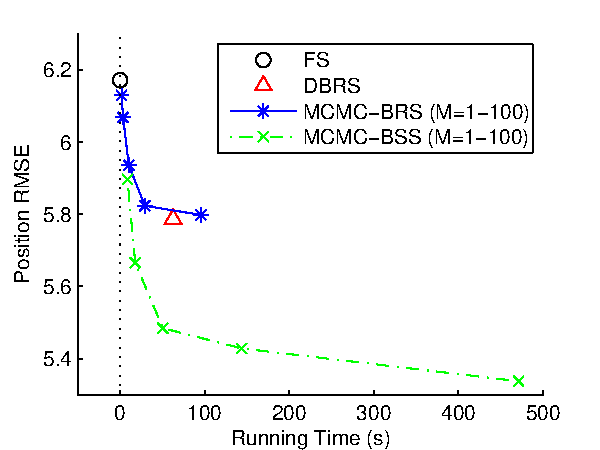
\includegraphics[width=0.45\columnwidth]{case2_smoother_comparison_posRMSE_time.pdf}}
\\
\subfloat[Case 3]{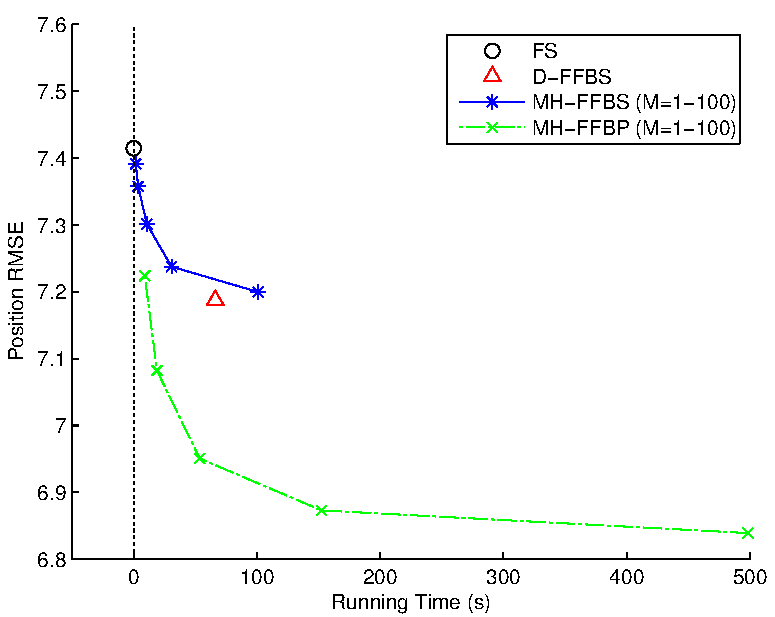
\includegraphics[width=0.45\columnwidth]{case3_smoother_comparison_posRMSE_time.pdf}}
\caption{Position RMSEs and running times of various smoothing algorithms with different noise covariance cases.}%
\label{fig:rmse_vs_time}%
\end{figure}

The MH-FFBS smoother error approaches that of the D-FFBS as the number of MH steps, $M$, increases. Similarly, the mean number of unique particles in the MH-FFBS approximation approaches that of the D-FFBS. This behaviour is expected as a longer Markov chain is more likely to deliver an independent sample from the target distribution, whereas independent samples are guaranteed in the D-FFBS approximation due to the direct sampling procedure.

When the number of MH steps, $M$, is small, the error of the MH-FFBS is often still significantly reduced relative to the D-FFBS but with a shorter running time. For a particular application, it is possible to adjust $M$ to control the trade-off between error and speed of computation. Thus, the MH-FFBS provides increased flexibility when compared to the D-FFBS scheme.

The MH-FFBP outperforms all of the other smoothers, achieving the lowest RMSE and ENEES for any given running time. Furthermore, because the support is not limited to using states from the filter distributions, the smoothing particle approximation has many more unique particles, giving a less degenerate representation.



\section{Conclusion} \label{sec:conclusions}
Two new algorithms have been presented for drawing particles from the joint smoothing distribution using Metropolis-Hastings. These MCMC schemes have a degree of flexibility in the choice of chain length, which controls a trade-off between accuracy and running time.

The first algorithm samples particles from the filtering approximations to produce particles from the smoothing distribution. The error performance of this scheme approaches that of the standard forward-filtering-backward-sampling of \cite{Godsill2004} as the chain length increases. However, comparable error performance may be achieved with very short chains, leading to a significant saving in processing time.

The second algorithm samples new values of the state from a continuous proposal density. Although slower than the previous scheme for a given length of Markov chain, the error performance is reduced relative to the other smoothers.



%\section{Appendix Title}
%Appendix one text goes here.



%\section*{Acknowledgment}
%The authors would like to thank...


\newpage
\bibliographystyle{IEEEtran}
\bibliography{D:/pb404/Dropbox/PhD/Cleanbib}

%\newpage

%\begin{IEEEbiography}[{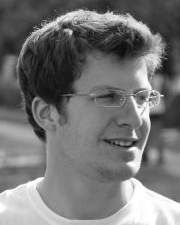
\includegraphics[width=1in,height=1.25in,clip,keepaspectratio]{Bunch-bw.jpg}}]{Pete Bunch} (M'11) has an MEng. degree from the University of Cambridge, UK, and is currently cogitating towards a PhD degree in signal processing at the Cambridge University Engineering Department.

He is an enthusiastic Bayesian, with research interests in sequential inference, Monte Carlo approximations and target tracking.
\end{IEEEbiography} 
%\begin{IEEEbiography}[{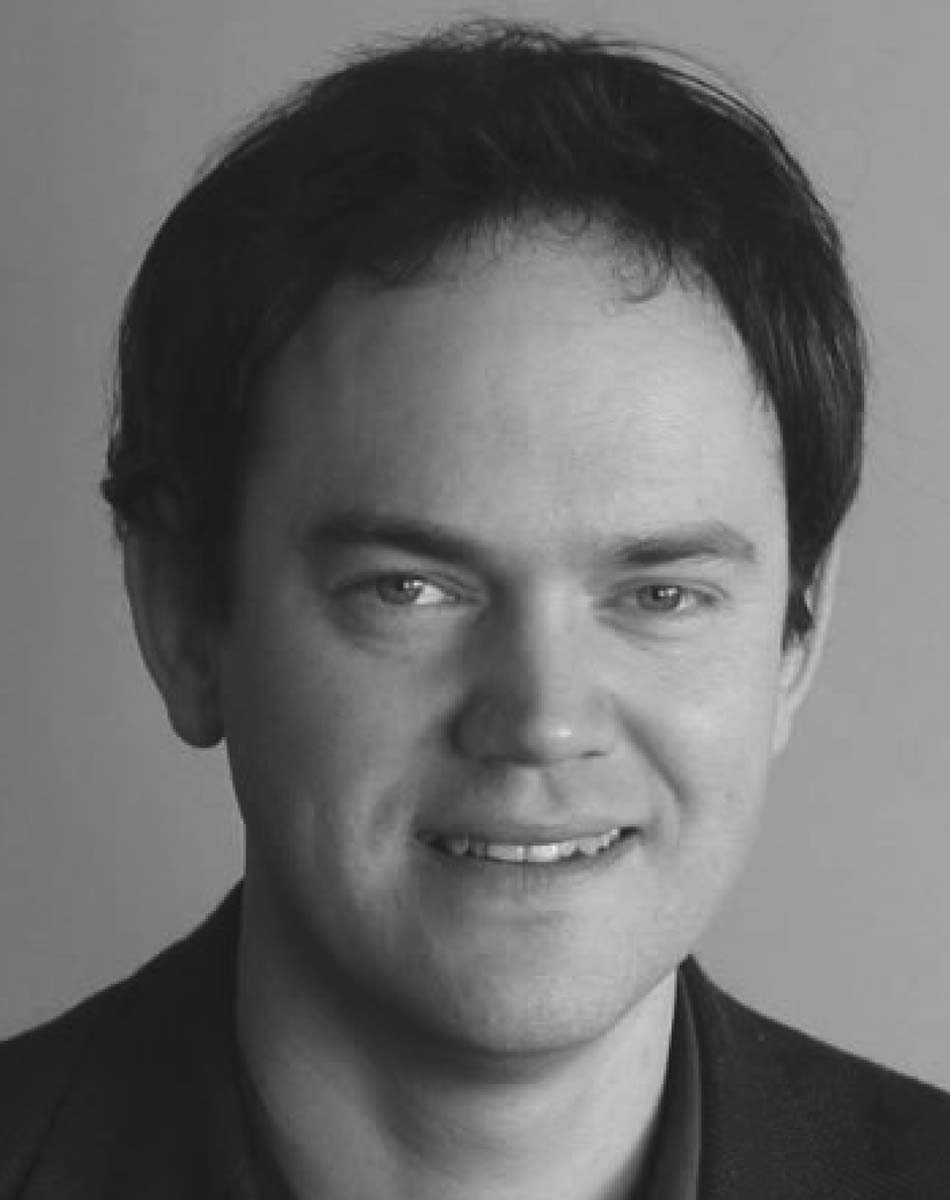
\includegraphics[width=1in,height=1.25in,clip,keepaspectratio]{Godsill.jpg}}]{Simon Godsill} is Professor of Statistical Signal Processing in the Engineering Department at Cambridge University and a Professorial Fellow and tutor at Corpus Christi College Cambridge.

He coordinates an active research group in Signal Inference and its Applications within the Signal Processing and Communications Laboratory at Cambridge, specialising in Bayesian computational methodology, multiple object tracking, audio and music processing, and financial time series modeling. A particular methodological theme over recent years has been the development of novel techniques  for optimal Bayesian filtering and smoothing, using Sequential Monte Carlo or Particle Filtering methods.

Prof. Godsill has published extensively in journals, books and international conference proceedings. He was technical chair of the IEEE NSSPW workshop in 2006 on sequential and nonlinear filtering methods, was Technical Chair for Fusion 2010 in Edinburgh, and has been on the conference panel for numerous other conferences and workshops. Prof. Godsill has served as Associate Editor for IEEE Tr. Signal Processing and the journal Bayesian Analysis. He was Theme Leader in Tracking and Reasoning over Time for the UK�s Data and Information Fusion Defence Technology Centre (DIF-DTC) and Principal Investigator on grants funded by the EU, EPSRC, QinetiQ, General Dynamics, MOD, Microsoft UK, Citibank and Mastercard. In 2009-10 he was co-organiser of an 18 month research program in Sequential Monte Carlo Methods at the SAMSI Institute in North Carolina. He is a Director of CEDAR Audio Ltd. (which has received a technical Oscar for its audio processing work), and Input Dynamics Ltd., both companies which use his research work in the audio area.   


\end{IEEEbiography} 

\end{document}


